\section{Durchführung}
\label{sec:Durchführung}

Bei diesem Versuch wir ein Röntgengerät, dargestellt in Abbildung 
\ref{fig:Aufbau}, verwendet. 

\begin{figure}
\centering
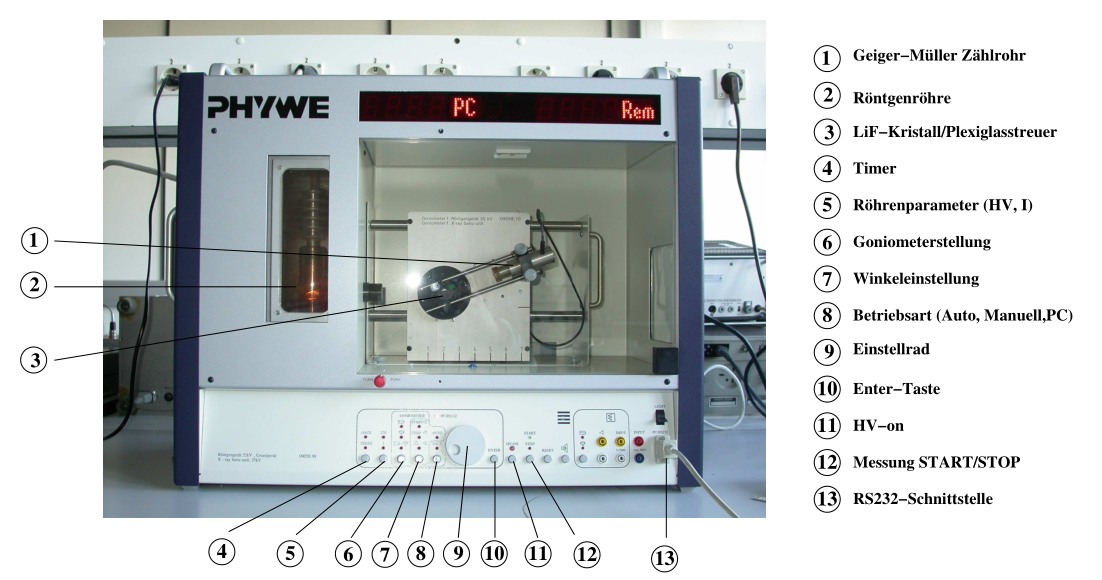
\includegraphics[scale=0.5]{content/aufbau1.png}
\caption{Röntgengerät. [1]}
\label{fig:Aufbau}
\end{figure}

Es besteht grundsätzlich aus einer Kupfer-Röntgen-Röhre, welche auf einen 
um sich selbst rotierbaren LiF-Kristall gerichtet ist. Auf einer Kreisbahn 
um den Kristall kann wiederrum ein auf jenen gerichtetes Geiger-Müller-Zählrohr
bewegt werden.
Diese Komponenten sind durch einen Computer miteinander verbunden und mit einer
dafür entwickelten Software steuerbar. Allerdings funktioniert das Gerät allerdings
auch ohne diesen Computer. Mit dieser Software können die Spannungs-
und Stromzufuhr der Röntgenröhre einzeln oder simultan festgelegt und variiert 
werden. Beispiel ist ein 2:1 Modus, dabei hat das Zählrohr den doppelten 
Winkel des Kristalls.
Zusätzlich können der Winkelzuwachs und die Integrationszeit, also die Zeit in der 
jeder Winkel gehalten werden soll, eingestellt werden. 
Außerdem nimmt die Software die Zählrate in Abhängigkeit des Winkels des Kristalls 
auf. Für die Messung der Absorptionsspektren können vor das Geiger-Müller-Zählrohr
Blenden mit verschiedenen Absorbern geschraubt werden. 
Es ist zu beachten, das Röntgengerät nur im geschlossenen Zustand laufen zu lassen. 

Bei jeder Untersuchung wird die Stromstärke auf $I = \SI{1}{\milli\ampere}$ und die 
Beschleunigungsspannung der Röntgenröhre auf $U = \SI{35}{\kilo\volt}$ gestellt. 

\subsection{Überprüfung der Bragg Bedingung}

Um die Bragg Bedingung zu überprüfen, wird zunächst der LiF-Kristall auf einen 
festen Winkel $\SI{14}{\degree}$ relativ zur Strahllinie gestellt. 
Das Zählrohr fährt den Winkelbereich von $\SI{26}{\degree}$ und $\SI{30}{\degree}$
in $\SI{0.1}{\degree}$-Schritten mit einer Integrationszeit von $\SI{20}{\second}$
ab. Somit liegt $\SI{14}{\degree}$ genau in diesem Bereich, da wir $2\theta$ betrachten, 
also $\SI{28}{\degree}$.

\subsection{Emissionsspektrum der Kupfer-Röntgen-Röhre}

Zum Messen des Emissionsspektrums und auch für die folgenden Messungen wird die 
Messmethode auf den 2:1 Koppel-Modus umgestellt. 
Die Drehung des Kristalls soll von $\SI{4}{\degree}$ bis $\SI{26}{\degree}$ 
stattfinden, diesmal jedoch in $\SI{0.2}{\degree}$-Schritten mti einer Integrationszeit
von $\SI{5}{\second}$.

\subsection{Absorptionsspektren}

Zunächst wird die Öffnung des Zählrohrs mit dem entsprechenden Absorber versehen. 
Die Messung erfolgt in $\SI{0.1}{\degree}$-Schritten mit einer Integrationszeit
von $\SI{20}{\second}$. Dabei wird versucht, den Teil des Spektrums aufzunehmen, 
in der die K-Kante zu sehen ist. 
Dies wird für Zink, Strontium, Brom und Zirkonium getan. 
Bei der letzten Messung mit Gold wird ein Spektrum aufgenommen, welches die ersten
drei L-Kanten beinhaltet, von denen allerdings nur die $L_\text{II}$- und 
$L_\text{I}$-Kante aufgelöst werden können. 